% !TeX root = er.tex

\chapter{Navigation locale : Évitement d'obstacles}\label{ch.obstacle}

Un robot mobile doit naviguer d'un point à un autre de son environnement. Il peut s'agir d'une tâche simple, par exemple si un robot peut suivre une ligne sans obstacle sur le sol d'un entrepôt (\ref{s.line}), mais la tâche devient plus difficile dans des environnements inconnus et complexes comme un rover explorant la surface de Mars ou un submersible explorant une chaîne de montagnes sous-marine. Même une voiture autonome qui circule sur une route doit faire face aux autres voitures, aux obstacles sur la route, aux passages pour piétons, à la construction des routes, etc. 

La navigation d'une voiture autonome peut être divisée en deux tâches : La première, de haut niveau, consiste à trouver un chemin entre une position de départ et une position d'arrivée. Avant le développement des systèmes informatiques modernes, pour trouver un chemin, il fallait étudier une carte ou demander son chemin. Aujourd'hui, il existe des applications pour smartphones qui prennent une position de départ et une position d'arrivée et calculent des chemins entre ces deux positions. Si l'application reçoit des données en temps réel sur les conditions de circulation, elle peut suggérer le chemin qui vous permettra d'atteindre votre objectif le plus rapidement possible. Le chemin peut être calculé hors ligne ou, si vous disposez d'un système GPS capable de déterminer votre position actuelle, le chemin peut être trouvé en temps réel et mis à jour pour tenir compte de l'évolution des conditions.

Une voiture autonome doit également adapter son comportement à l'environnement : s'arrêter pour laisser passer un piéton sur un passage piéton, tourner aux intersections, éviter les obstacles sur la route, etc. Alors que la recherche de chemin de haut niveau peut être effectuée une fois avant le voyage (ou toutes les quelques minutes), la tâche de bas niveau consistant à éviter les obstacles doit être exécutée fréquemment, car la voiture ne sait jamais quand un piéton va sauter sur la route ou quand la voiture qu'elle suit va soudainement freiner.

La section~\ref{s.obstacle-avoidance} examine la tâche de bas niveau d'évitement des obstacles. La section~\ref{s.no-localization} montre comment un robot peut reconnaître des marquages tout en suivant une ligne afin de savoir quand il a atteint son objectif. Les sections~\ref{s.ants}--\ref{s.fsm-ants} démontrent un comportement de plus haut niveau : trouver un chemin sans carte de l'environnement. Cela se fait par analogie avec une colonie de fourmis localisant une source de nourriture et communiquant son emplacement à tous les membres de la colonie.

\section{Evitement des obstacles}\label{s.obstacle-avoidance}
\index{évitement des obstacles}

Les algorithmes présentés jusqu'à présent se sont concentrés sur la détection d'objets et le déplacement vers ceux-ci. Lorsqu'un robot se déplace vers un objectif, il est susceptible de rencontrer des objets supplémentaires appelés \emph{obstacles} qui bloquent le chemin et empêchent le robot d'atteindre son objectif. Nous supposons que le robot est capable de détecter s'il existe un chemin libre vers l'objectif, par exemple en détectant une lumière sur l'objectif. Cette section décrit trois algorithmes d'évitement d'obstacles, où les obstacles sont des murs qui bloquent le mouvement du robot :
\begin{itemize}
\item Un algorithme simple de suivi de mur, qui malheureusement ne fonctionnera pas s'il y a plusieurs obstacles dans l'environnement.
\item Un algorithme qui peut éviter plusieurs obstacles, mais qui doit connaître la direction générale du but (peut-être grâce à son système GPS). Malheureusement, certains obstacles peuvent bloquer le robot dans une boucle.
\item L'algorithme Pledge est une petite modification du second qui permet de surmonter ce comportement erroné.
\end{itemize}
Les algorithmes utilisent les expressions conditionnelles abstraites \p{mur devant} et \p{mur à droite}, qui sont vraies si un mur se trouve à l'avant ou à la droite du robot. Le premier algorithme utilisera également l'expression conditionnelle \p{corner-right} qui est vraie si le robot se déplace autour d'un obstacle et détecte un coin à sa droite. Il existe plusieurs façons d'implémenter ces expressions, que nous étudions dans Activity~\ref{act.wall-expressions}.

\begin{framed}
\act{Expressions conditionnelles pour suivre un mur}{wall-expressions}
\begin{itemize}
\item Mettre en œuvre l'expression conditionnelle \p{suivi du mur} à l'aide d'un capteur de proximité horizontal ou d'un capteur tactile.
\item Mettre en œuvre l'expression conditionnelle \p{wall-right}. Ceci est facile à réaliser avec un capteur monté à droite du robot, ou avec un capteur de distance rotatif. Si vous n'avez qu'un capteur de proximité orienté vers l'avant, vous pouvez demander au robot de se tourner légèrement vers la droite, de détecter le mur, s'il y en a un, puis de faire demi-tour.
\item Mettre en œuvre l'expression conditionnelle \p{coin-droit}. Elle peut être mise en œuvre comme une extension de \p{mur-droit}. Lorsque la valeur de \p{wall-right} passe de vrai à faux, effectuer un court virage à droite et vérifier si \p{wall-right} redevient vrai.
\end{itemize}
\end{framed}

\subsection{suivi du mur}
\index{mur suivant}

La figure~\ref{fig.wall-following-simple} montre un robot qui suit un mur en maintenant sa position de manière à ce que le mur soit à sa droite (Algorithme~\ref{alg.wall-following-simple}). Si un mur est détecté devant lui, le robot tourne à gauche de manière à ce que le mur soit à sa droite. Si un mur est détecté à droite, le robot continue à se déplacer le long du mur. Si un coin est détecté, le robot tourne à droite pour continuer à contourner l'obstacle. En même temps, le robot cherche continuellement le but (point noir). Lorsqu'il détecte l'objectif, le robot se déplace directement vers lui.

\begin{figure}
\begin{center}
\begin{tikzpicture}[scale=.7]
\draw[fill,color=gray] (4,0) rectangle +(4,.8);
\draw[fill,color=gray] (5,0) rectangle +(.8,-1);
\pic[rotate=90,scale=.5] at (7,-3) { robot };
\draw[fill] (6,4) node[right,xshift=4pt] {\p{Objectif}} circle[radius=4pt];
\draw[->] (7,-2) -- ++(90:1.8) -- ++(180:1) -- ++(-90:1) -- ++(180:1.2) -- ++(90:1) -- ++(180:1) -- ++(90:1.2) coordinate(corner);
\draw[dashed,->] (corner) -- (5.9,3.9);
\path (-.3,0);  % Extra space so arrow isn't chopped
\end{tikzpicture}
\caption{Suivi du mur}\label{fig.wall-following-simple}
\end{center}
\end{figure}

\begin{figure}
\begin{alg}{Simple suivi du mur}{wall-following-simple}
\hline
\stl{}&while not-at-goal&\\
\stl{}&\idc{}if goal-detected&\\
\stl{}&\idc{}\idc{}move towards goal&\\
\stl{}&\idc{}else if wall-ahead&\\
\stl{}&\idc{}\idc{}turn left&\\
\stl{}&\idc{}else if corner-right&\\
\stl{}&\idc{}\idc{}turn right&\\
\stl{}&\idc{}else if wall-right&\\
\stl{}&\idc{}\idc{}move forward&\\
\stl{}&\idc{}else&\\
\stl{}&\idc{}\idc{}move forward&\\
\end{alg}
\end{figure}

Malheureusement, l'algorithme~\ref{alg.wall-following-simple} ne fonctionne pas toujours correctement. La figure~\ref{fig.wall-following-simple-bug} montre une configuration avec \emph{deux} obstacles entre le robot et le but. Le robot ne détectera jamais l'objectif et se déplacera donc indéfiniment autour du premier obstacle.

\begin{framed}
\act{Simple suivi de mur}{simple-wall-following}
\begin{itemize}
\item Mettre en œuvre l'algorithme~\ref{alg.wall-following-simple} et vérifier qu'il démontre les comportements montrés dans les Figs.\ref{fig.wall-following-simple}, \ref{fig.wall-following-simple-bug}.\ref{fig.wall-following-simple-bug}.
\end{itemize}
\end{framed}

\begin{figure}
\begin{center}
\begin{tikzpicture}[scale=.8]
\draw[fill,color=gray] (4,0) rectangle +(4,.8);
\draw[fill,color=gray] (5,0) rectangle +(.8,-1);
\draw[fill,color=gray] (0,2) rectangle +(9,.8);
\draw[fill,color=gray] (1.5,2) rectangle +(.8,-1);
\pic[rotate=90,scale=.5] at (7,-3) { robot };
\draw[fill] (6,4) node[right,xshift=4pt] {\p{Objectif}} circle[radius=4pt];
\draw[->] (7,-2) -- ++(90:1.8) -- ++(180:1) -- ++(-90:1) -- ++(180:1.2) -- ++(90:1) -- ++(180:1) -- ++(90:1.2) coordinate(corner) -- ++(0:4.4) -- ++(-90:1.2) -- ++(180:1);
\draw[dashed,->] (corner) -- (5.9,3.9);
\path (-.3,0);  % Extra space so arrow isn't chopped
\end{tikzpicture}
\caption{Le simple suivi du mur ne permet pas toujours au robot d'atteindre l'objectif}\label{fig.wall-following-simple-bug}
\end{center}
\end{figure}

\subsection{Suivi de mur avec direction}
\index{suivi de mur!direction@avec direction}

Le problème de l'algorithme~\ref{alg.wall-following-simple} est qu'il s'agit d'un algorithme local qui ne regarde que son environnement immédiat et ne tient pas compte du fait que l'algorithme de navigation de niveau supérieur connaît approximativement la direction que le robot doit prendre pour atteindre l'objectif. La figure \ref{fig.wall-following-direction} montre le comportement d'un robot qui "sait" que le but se trouve quelque part au nord et qui se déplace donc à un cap de $0^\circ$ par rapport au nord. L'algorithme de suivi de mur n'est utilisé que si le robot ne peut pas se déplacer vers le nord.

\begin{figure}
\begin{center}
\begin{tikzpicture}[scale=.7]
\draw[fill,color=gray] (4,0) rectangle +(4,.8);
\draw[fill,color=gray] (5,0) rectangle +(.8,-1);
\draw[fill,color=gray] (0,2) rectangle +(9,.8);
\draw[fill,color=gray] (1.5,2) rectangle +(.8,-1);
\pic[rotate=90,scale=.5] at (7,-3) { robot };
\draw[fill] (6,4) node[right,xshift=4pt] {\p{Objectif}} circle[radius=4pt];
\draw[->] (7,-2) -- ++(90:1.8) -- ++(180:1) -- ++(-90:1) -- ++(180:1.2) -- ++(90:1) -- ++(180:1) -- ++(90:2) -- ++(180:1.3) -- ++(-90:1) -- ++(180:1.2) -- ++(90:1) -- ++(180:1.5) -- ++(90:1.4) coordinate(corner);
\draw[dashed,->] (corner) -- (5.8,4);
\path (-.3,0);  % Extra space so arrow isn't chopped
\end{tikzpicture}
\caption{Mur qui suit la direction}\label{fig.wall-following-direction}
\end{center}
\end{figure}

L'algorithme \ref{alg.wall-follow} est similaire à l'algorithme précédent, à l'exception du fait qu'il préfère se déplacer vers le nord si possible. Il utilise une variable \p{heading} pour se souvenir de son cap actuel lorsqu'il se déplace autour de l'obstacle. Lorsque \p{heading} est à nouveau au nord (un multiple de $360^\circ$), le robot avance au lieu de chercher un coin.

\begin{figure}
\begin{alg}{Suivi des murs}{wall-follow}
&\idv{}integer heading \ass $0^\circ$&\\
\hline
\stl{}&while not-at-goal&\\
\stl{}&\idc{}if goal-detected&\\
\stl{}&\idc{}\idc{}move towards goal&\\
\stl{}&\idc{}else if wall-ahead&\\
\stl{}&\idc{}\idc{}turn left&\\
\stl{}&\idc{}\idc{}heading \ass heading $+\: 90^\circ$&\\
\stl{}&\idc{}else if corner-right&\\
\stl{}&\idc{}\idc{}if heading $=$ multiple of $360^\circ$&\\
\stl{}&\idc{}\idc{}\idc{}move forward&\\
\stl{}&\idc{}\idc{}else&\\
\stl{}&\idc{}\idc{}\idc{}turn right&\\
\stl{}&\idc{}\idc{}\idc{}heading \ass heading $-\: 90^\circ$&\\
\stl{}&\idc{}else if wall-right&\\
\stl{}&\idc{}\idc{}move forward&\\
\stl{}&\idc{}else&\\
\stl{}&\idc{}\idc{}move forward&\\
\end{alg}
\end{figure}

Malheureusement, l'algorithme peut échouer lorsqu'il est confronté à un obstacle en forme de \ref{fig.wall-direction-bug}). Après avoir effectué quatre virages à gauche, il se dirige vers $360^\circ$ (également vers le nord, un multiple de $360^\circ$) et continue d'avancer, rencontrant et suivant le mur encore et encore.

\begin{figure}
\begin{center}
\begin{tikzpicture}[scale=.7]
\draw[fill,color=gray] (0,0) rectangle +(4,.8);
\draw[fill,color=gray] (3.2,0) rectangle +(.8,1.5);
\draw[fill,color=gray] (0,0) rectangle +(.8,4);
\draw[fill,color=gray] (0,3.2) rectangle +(6,.8);
\pic[rotate=90,scale=.5] at (5.2,.3) { robot };
\draw[->] (5.2,1.1) -- ++(90:1.9) -- ++(180:4.2) -- ++(-90:2) -- ++(0:2) -- ++(90:1.6);
\draw[->,thick] (-1,1) -- node[left,xshift=-4pt] {\p{Objectif}} +(0,2);
\end{tikzpicture}
\caption{Pourquoi le suivi d'un mur avec direction ne fonctionne pas toujours}\label{fig.wall-direction-bug}
\end{center}
\end{figure}

\begin{framed}
\act{Suivi du mur avec direction}{wall-following}
\begin{itemize}
\item Mettre en oeuvre l'algorithme de suivi de mur avec direction et vérifier qu'il démontre le comportement montré dans la Fig.~\ref{fig.wall-direction-bug}.
\item Exécuter l'algorithme de suivi de mur simple (Algorithm~\ref{alg.wall-following-simple}) avec un obstacle en forme de \emph{G}. Que se passe-t-il ? Cela affecte-t-il notre affirmation selon laquelle cet algorithme n'est pas adapté à l'évitement d'obstacles ?
\end{itemize}
\end{framed}

\subsection{L'algorithme de l'engagement}
\index{suivi de mur!algorithme de gage}

L'algorithme de gage modifie la ligne~8 de l'algorithme de suivi de mur en :
\begin{quote}
\normalsize \p{if heading $= 0^\circ$}
\end{quote}
Le robot n'avance que lorsque son cap cumulé est égal à $0^\circ$ et non lorsqu'il se déplace vers le nord--un cap qui est un multiple de $360^\circ$. Le robot évite maintenant l'obstacle en forme de "G" (Fig.~\ref{fig.wall-following-pledge}) : lorsqu'il rencontre le coin (point noir), il se déplace vers le nord, mais son cap est de $360^\circ$ après quatre virages à gauche. Bien que $360^\circ$ soit un multiple de $360^\circ$, il n'est pas égal à $0^\circ$. Par conséquent, le robot continue à suivre le mur jusqu'à ce que quatre virages à droite soustraient $360$, de sorte que le cap total est de $0^\circ$.

\begin{figure}
\begin{center}
\begin{tikzpicture}[scale=.7]
\draw[fill,color=gray] (0,0) rectangle +(4,.8);
\draw[fill,color=gray] (3.2,0) rectangle +(.8,1.5);
\draw[fill,color=gray] (0,0) rectangle +(.8,4);
\draw[fill,color=gray] (0,3.2) rectangle +(6,.8);
\pic[rotate=90,scale=.5] at (5.2,.3) { robot };
\draw[->] (5.2,1.1) -- ++(90:1.9) -- ++(180:4.2) -- ++(-90:2) -- ++(0:2) -- ++(90:.7) -- ++(0:1.2) -- ++(-90:1.9) -- ++(180:4.4) -- ++(90:4.5);
\fill (3.2,1.5) circle [radius=3pt];
\draw[->,thick] (-1,1) -- node[left,xshift=-4pt] {\p{Objectif}} +(0,2);
\path (-.3,0);  % Extra space so arrow isn't chopped
\end{tikzpicture}
\caption{Algorithme de promesse de suivi du mur}\label{fig.wall-following-pledge}
\end{center}
\end{figure}

\begin{framed}
\act{Algorithme de Pledge}{pledge-algorithm}
\begin{itemize}
\item Mettre en œuvre l'algorithme de promesse et vérifier qu'il présente le comportement illustré dans la Fig.~\ref{fig.wall-following-pledge}.
\end{itemize}
\end{framed}

\section{Suivre une ligne avec un code}\label{s.no-localization}
\index{suivre une ligne avec un code}

Revenons à la tâche qui consiste à trouver un chemin vers un but. Si le chemin est marqué par une ligne sur le sol, les algorithmes de suivi de ligne (Sect.~\ref{s.line}) peuvent guider un robot dans l'environnement, mais le suivi de ligne n'est pas de la navigation. Pour naviguer d'une position à l'autre, nous avons également besoin d'un algorithme de localisation afin que le robot sache quand il a atteint ses objectifs. Nous n'avons pas besoin d'un algorithme de localisation continue comme ceux du chapitre \ref{ch.local}, nous avons seulement besoin de connaître les positions sur la ligne qui facilitent l'accomplissement de la tâche. Cela ressemble à la navigation en voiture : il suffit de connaître les échangeurs, les intersections, les principaux points de repère, etc. pour savoir où l'on se trouve. Entre ces positions, il suffit de suivre la route.

La navigation sans localisation continue peut être mise en œuvre en lisant un code placé sur le sol à côté de la ligne. La figure \ref{fig.code-line} montre un robot équipé de deux capteurs au sol : celui de gauche détecte la ligne et celui de droite le code. Sous le robot se trouve un graphique du signal renvoyé par le capteur de droite.

\begin{figure}
\begin{center}
\begin{tikzpicture}
\draw[fill,lightgray] (-1,-4mm) rectangle +(8,5mm);
\pic[scale=1.2] at (0,-7mm) { robot2 };
\draw[fill,lightgray] (20mm,-14mm) rectangle +(4mm,6mm);
\draw[fill,lightgray] (30mm,-14mm) rectangle +(8mm,6mm);
\draw[fill,lightgray] (50mm,-14mm) rectangle +(4mm,6mm);
\draw[very thick,rounded corners] (-10mm,-30mm) -- ++(29mm,0mm) -- ++(2mm,8mm) -- ++(3mm,0mm) -- ++(2mm,-8mm) -- ++(3mm,0mm) -- ++(2mm,8mm) -- ++(6mm,0mm) -- ++(2mm,-8mm) -- ++(10mm,0mm) -- ++(2mm,8mm) -- ++(3mm,0mm) -- ++(2mm,-8mm) -- ++(12mm,0mm);
\node at (4mm,-26mm) {\p{sortie du capteur droit}}; 
\end{tikzpicture}
\end{center}
\caption{Un robot suit une ligne avec son capteur gauche et lit un code avec son capteur droit}\label{fig.code-line}
\end{figure}

\begin{framed}
\act{Suivre une ligne tout en lisant un code}{line-coded}
\begin{itemize}
\item Mettre en oeuvre le suivi de ligne avec la lecture de code comme indiqué sur la Fig.~\ref{fig.code-line}.
\item Ecrire un programme qui permet à un robot de suivre un chemin.
\item Placer des marques qui codent des valeurs à côté du chemin. Le robot doit afficher ces valeurs (à l'aide de la lumière, du son ou d'un écran) lorsqu'il se déplace sur les codes.
\end{itemize}
\end{framed}

\begin{framed}
\act{Suivi de ligne circulaire lors de la lecture d'un code}{line-coded-circular}
\begin{itemize}
\item Mettre en place une horloge en utilisant deux robots, l'un pour les minutes et l'autre pour les heures (Fig.~\ref{fig.line-clock}).
\item Une autre solution consisterait à faire en sorte que les deux robots se déplacent à des vitesses différentes, de sorte que l'un d'eux effectue une révolution en une heure et l'autre en un jour. Discutez de la différence entre ces deux implémentations.
\end{itemize}
\end{framed}

\begin{figure}
\begin{center}
\begin{tikzpicture}[scale=.8]
\begin{scope}[lightgray,line width=2.5mm]
\draw (0,0) circle[radius=44mm];
\foreach \n in {12, 1, 2, 3, 4, 5, 6, 7, 8, 9, 10, 11} {
  \node at (\n*30:51mm) [rectangle,fill,draw,rotate=\n*30] {};
  \node[black] at (90-\n*30:56mm) {\p{\n}};
}
\draw[lightgray] (0,0) circle[radius=20mm];
\foreach \n in {12, 1, 2, 3, 4, 5, 6, 7, 8, 9, 10, 11} {
  \node at (\n*30:27mm) [rectangle,fill,draw,rotate=\n*30] {};
  \node[black] at (90-\n*30:32mm) {\p{\n}};
}
\node at (0,0) [rectangle,fill,draw,minimum width=8mm,inner sep=1pt] {};
\node at (0,0) [rectangle,fill,draw,minimum height=8mm,inner sep=1pt] {};
\end{scope}
\pic[scale=.7,rotate=279] at (15:23mm) { robot2 };
\pic[scale=.7,rotate=-50] at (46:48mm) { robot2 };
\end{tikzpicture}
\end{center}
\caption{Une horloge robotisée : un robot indique l'heure et l'autre les minutes.}\label{fig.line-clock}
\end{figure}

\section[Fourmis à la recherche de la nourriture]{Fourmis à la recherche d'une source de nourriture}\label{s.ants}
\index{recherche de chemin!fourmis}

Revenons maintenant à l'algorithme de haut niveau de recherche d'un chemin. S'il existe une ligne et un mécanisme de localisation comme un code, l'approche de la section précédente peut être utilisée. Cependant, même si une ligne n'existe pas, un robot peut être capable de créer sa propre ligne. L'aspect intéressant de cette méthode est que le robot n'a pas besoin de connaître sa position dans l'environnement, par exemple à l'aide d'un GPS ; au lieu de cela, il utilise des points de repère dans l'environnement lui-même pour la navigation. L'algorithme sera présenté dans le contexte réel des fourmis à la recherche de nourriture :

\begin{quote}
\normalsize Il existe un nid de fourmis. Les fourmis cherchent au hasard une source de nourriture. Lorsqu'une fourmi trouve de la nourriture, elle retourne directement au nid en utilisant des points de repère et sa mémoire du chemin qu'elle a emprunté depuis le nid. Pendant le trajet de retour au nid avec la nourriture, la fourmi dépose des substances chimiques appelées \emph{phéromones}. Au fur et à mesure que les fourmis trouvent la source de nourriture et retournent au nid, la piste accumule plus de phéromones que les autres zones visitées par les fourmis. Finalement, la quantité de phéromones sur la piste est si importante que les fourmis peuvent suivre un chemin direct du nid à la source de nourriture.
\end{quote}

La figure~\ref{fig.ant-nest-food} montre le nid des fourmis dans le coin inférieur gauche représenté par une lumière qui permet aux fourmis de retrouver facilement leur chemin vers le nid. Le point sombre est la source de nourriture. La figure~\ref{fig.ant-nest-food-trail} montre trois pistes aléatoires qui finissent par découvrir la source de nourriture ; les fourmis retournent alors directement au nid, laissant trois lignes droites de phéromones. Cette concentration peut être utilisée ultérieurement pour trouver directement la source de nourriture.

\begin{figure}
\begin{minipage}{.45\textwidth}
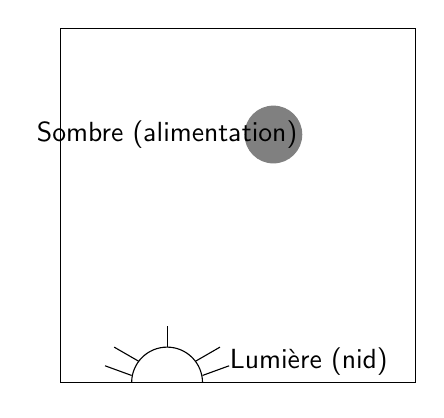
\begin{tikzpicture}[scale=.9]
% Light and dark with labels
\draw (0,0) -- (5,0) -- (5,5) -- (0,5) -- cycle;
\draw (2,0) arc[start angle=0, end angle=180, radius=5mm];
\node at (3.5,.3) {\textsf{Lumière (nid)}};
\draw (19mm,3mm) -- +(30:4mm);
\draw (20mm,1mm) -- +(20:4mm);
\draw (11mm,3mm) -- +(150:4mm);
\draw (10mm,1mm) -- +(160:4mm);
\draw (15mm,5mm) -- (15mm,8mm);
\draw[fill,gray] (3,3.5) circle[radius=4mm];
\node at (1.5,3.5) {\textsf{Sombre (alimentation)}};
\path (0,-.1) -- (5,-.1); % To prevent truncation
\end{tikzpicture}
\caption{Le nid de fourmis et la source de nourriture}\label{fig.ant-nest-food}
\end{minipage}
\hspace{\fill}
\begin{minipage}{.45\textwidth}
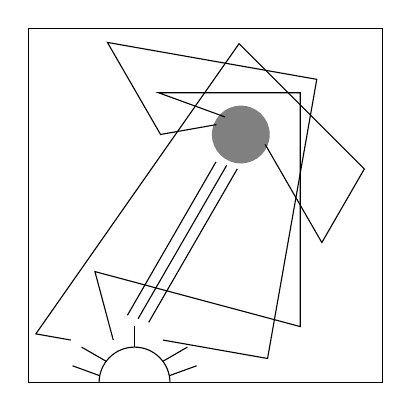
\begin{tikzpicture}[scale=.9]
\draw (0,0) -- (5,0) -- (5,5) -- (0,5) -- cycle;
\draw (2,0) arc[start angle=0, end angle=180, radius=5mm];
\draw (19mm,3mm) -- +(30:4mm);
\draw (20mm,1mm) -- +(20:4mm);
\draw (11mm,3mm) -- +(150:4mm);
\draw (10mm,1mm) -- +(160:4mm);
\draw (15mm,5mm) -- (15mm,8mm);
\draw[fill,gray] (3,3.5) circle[radius=4mm];
% Straight lines between light and dark
\begin{scope}[xshift=-1mm,yshift=2mm]
%\draw (13.5mm,8mm) -- +(60:2.5);
\draw (15mm,7.5mm) -- +(60:2.5);
\draw (16.5mm,7mm) -- +(60:2.5);
\draw (18mm,6.5mm) -- +(60:2.5);
\end{scope}
% Random lines between light and dark
\draw (19mm,6mm) -- ++(-10:15mm) -- ++(80:40mm) -- ++(170:30mm) -- ++(-60:15mm) -- ++(10:8mm);
\draw (12mm,6mm) -- ++(-75:-10mm) -- ++(-15:30mm) -- ++(90:33mm) -- ++(180:20mm) -- ++(-20:10mm);
\draw (6mm,6mm) -- ++(170:5mm) -- ++(55:50mm) -- ++(-45:25mm) -- ++(-120:12mm) -- ++(120:16mm);
\path (0,-.1) -- (5,-.1); % To prevent truncation
\end{tikzpicture}
\caption{Les phéromones\\créent une piste}\label{fig.ant-nest-food-trail}
\end{minipage}
\end{figure}

Le comportement de la fourmi peut être mis en œuvre par un robot.\label{s.ant-like-algo} Supposons qu'il existe une zone fixe à l'intérieur de laquelle le robot peut se déplacer. Comme dans la Fig.~\ref{fig.ant-nest-food}, il y a une source de nourriture et un nid. La source de nourriture est représentée par un point sombre qui peut être facilement détecté par un capteur au sol du robot. Les capteurs de proximité du robot sont utilisés pour détecter les murs de la zone. \ref{act.locate-nest} propose deux méthodes de représentation du nid qui dépendent des capteurs supplémentaires dont dispose votre robot.

\begin{framed}
\act{Localiser le nid}{locate-nest}
\begin{itemize}
\item Mettre en œuvre un programme qui oblige le robot à se déplacer vers le nid, quel que soit l'endroit où il est placé dans la zone.
\item Accéléromètres : Monter la zone sur une pente de telle sorte qu'un coin, le nid, se trouve au point le plus bas de la zone. 
\item Capteur de lumière : Le nid est représenté par une source de lumière qui peut être détectée par le capteur de lumière indépendamment de la position et de la direction du robot. Si le capteur de lumière est fixe et ne peut détecter la lumière que dans une certaine direction, le robot devra tourner pour localiser la source de lumière.
\end{itemize}
\end{framed}

Simulez les phéromones en recouvrant la zone d'une feuille de papier blanc et en attachant un marqueur noir au robot de manière à ce qu'il trace une ligne partout où il se déplace. Un capteur au sol détecte les marques dans la zone. La figure~\ref{fig.ant-result} montre les lignes résultant du comportement d'un robot exécutant l'algorithme. L'activité~\ref{act.high-density} vous demande d'explorer la capacité du robot à détecter les zones présentant une forte densité de lignes.

\begin{figure}
\begin{center}
\includegraphics[width=.8\textwidth]{density-map-0}
\end{center}
\caption{Un robot simulant les phéromones des fourmis}\label{fig.ant-result}
\end{figure}

\begin{framed}
\act{Détection des zones de haute densité}{high-density}
\begin{itemize}
\item Dans la section \ref{s.no-gradient}, nous avons noté que les capteurs ne détectent pas un seul point géométrique mais ont plutôt une ouverture qui lit une zone relativement grande, peut-être même jusqu'à un centimètre carré (\ref{fig.no-gradient}). Faites des expériences avec votre capteur au sol pour voir comment les lectures renvoyées par le capteur dépendent de la largeur de la ligne. Pouvez-vous tirer une conclusion sur la largeur optimale du marqueur ? S'il est trop fin, la piste ne sera pas détectée et s'il est trop épais, les marques du mouvement aléatoire pourraient être prises pour la piste.
\item Représentez la source de nourriture comme une tache relativement grande et totalement noire et assurez-vous qu'elle donne une lecture minimale du capteur au sol.
\item La figure~\ref{fig.ant-result} montre que la piste entre la source de nourriture et le nid a une densité élevée. Expérimentez avec différents nombres de lignes et définissez un seuil efficace entre la piste et les zones de mouvement aléatoire à l'extérieur de la piste. Voyez si vous pouvez faire en sorte que le robot trace des lignes plus foncées en variant son mouvement ou en se déplaçant d'avant en arrière le long de la piste.
\end{itemize}
\end{framed}


\section[Un modèle probabiliste]{Un modèle probabiliste du comportement des fourmis}\label{s.ant-probabilistic}
\index{Recherche de chemin!modèle probabiliste des fourmis}

Un \emph{modèle} est une abstraction d'un système qui montre comment les paramètres influencent les phénomènes. Les modèles sont utilisés, par exemple, pour étudier les schémas de circulation afin de prédire l'effet de nouvelles routes ou de nouveaux feux de circulation. Pour comprendre comment le chemin entre le nid et la nourriture est généré, cette section présente un modèle simplifié du comportement des fourmis. 

La caractéristique fondamentale du comportement des fourmis est qu'elles ne disposent pas d'une carte de leur environnement et qu'elles doivent donc se déplacer au hasard pour rechercher la source de nourriture. Par conséquent, un modèle de leur comportement doit être probabiliste. Supposons que l'environnement soit une zone rectangulaire constituée d'une grille de cellules. La figure~\ref{fig.ant-grid-empty} montre une zone divisée en $6\times 8=48$ cellules.

\begin{quote}
\begin{center}
\textbf{Coordonnées dans une grille de cellules}
\end{center}
Tout au long du livre, les coordonnées d'une cellule dans une grille sont données sous la forme $(\textit{row}, \textit{column})$. Les lignes sont numérotées de haut en bas et les colonnes de gauche à droite, comme les matrices en mathématiques, mais la numérotation commence à partir de $0$, comme dans le type de données array en informatique.
\end{quote}

\begin{figure}
\begin{center}
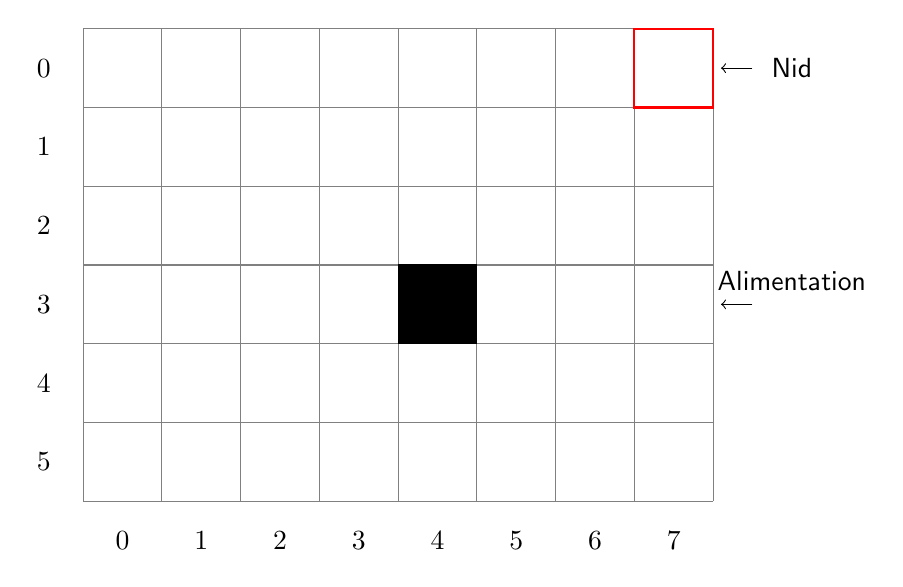
\begin{tikzpicture}
\draw[step=1cm,gray,thin] (0,0) grid (8,6);
\foreach \n/\x in {0/.5, 1/1.5, 2/2.5, 3/3.5, 4/4.5, 5/5.5, 6/6.5, 7/7.5}
  \node at (\x, -.5) {\p{\n}};
\foreach \n/\y in {5/.5, 4/1.5, 3/2.5, 2/3.5, 1/4.5, 0/5.5}
  \node at (-.5, \y) {\p{\n}};
\draw[fill] (4,2) rectangle +(1,1);
\node at (9,2.8) {\textsf{Alimentation}};
\draw[->] (8.5,2.5) to +(-.4,0);
\node at (9,5.5) {\textsf{Nid}};
\draw[->] (8.5,5.5) to +(-.4,0);
\draw[red,thick] (7,5) rectangle +(1,1);
\end{tikzpicture}
\end{center}
\caption{Représentation de l'environnement sous forme de grille de cellules}\label{fig.ant-grid-empty}
\end{figure}
Sans aucune information sur la façon dont les fourmis choisissent leurs mouvements, nous supposons qu'elles peuvent se déplacer dans n'importe quelle direction avec la même probabilité. La probabilité $p$ qu'une fourmi se trouve dans une cellule est donc égale à $1$ divisé par le nombre de cellules, soit ici $p=1/48=0,021$.

La probabilité que la fourmi se trouve dans la cellule où se trouve la source de nourriture est $p$, la même que pour toute autre cellule. Selon notre spécification du comportement de la fourmi, une fois qu'elle est entrée dans cette cellule et qu'elle a identifié la cellule comme étant la source de nourriture, elle retourne directement au nid. Dans la figure \ref{fig.ant-grid-empty}, la source de nourriture se trouve dans la cellule $(3,4)$, de sorte qu'une fourmi visitant cette cellule doit retourner au nid à la cellule $(0,7)$, en passant par les cellules $(2,5)$ et $(1,6)$. Quelle est la probabilité que la fourmi se trouve dans l'une de ces trois cellules ? Il y a deux possibilités : soit la fourmi est dans la cellule parce qu'elle s'y est déplacée au hasard avec une probabilité $p$, soit la fourmi s'y trouve parce qu'elle s'est déplacée vers la source de nourriture au hasard avec une probabilité $p$ et ensuite \emph{avec une probabilité $1$} s'est déplacée vers le nid. Par conséquent, la probabilité totale de se trouver dans l'une de ces cellules est de $p+p\times 1=p+p=2p$.\footnote{Après la mise à jour des probabilités, celles-ci doivent être normalisées comme expliqué dans l'annexe~\ref{a.normalize}. Pour un autre exemple de normalisation, voir la section~\ref{s.prob-local}.}  Si notre robot dessine des lignes en se déplaçant, les cellules situées sur la diagonale doivent être deux fois plus sombres que les autres cellules.

\begin{figure}
\begin{center}
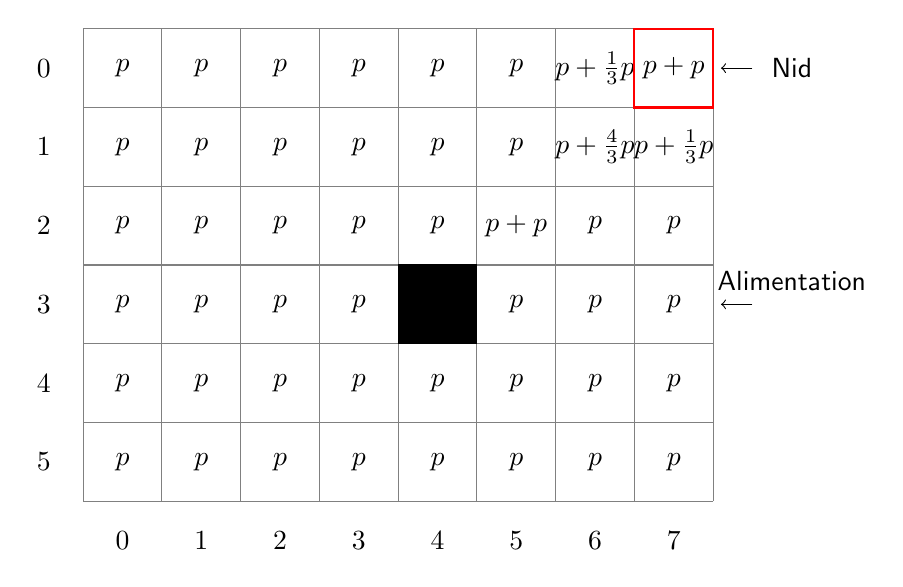
\begin{tikzpicture}
\draw[step=1cm,gray,thin] (0,0) grid (8,6);
\foreach \n/\x in {0/.5, 1/1.5, 2/2.5, 3/3.5, 4/4.5, 5/5.5, 6/6.5, 7/7.5}
  \node at (\x, -.5) {\p{\n}};
\foreach \n/\y in {5/.5, 4/1.5, 3/2.5, 2/3.5, 1/4.5, 0/5.5}
  \node at (-.5, \y) {\p{\n}};
\draw[fill] (4,2) rectangle +(1,1);
\node at (9,2.8) {\textsf{Alimentation}};
\draw[->] (8.5,2.5) to +(-.4,0);
\node at (9,5.5) {\textsf{Nid}};
\draw[->] (8.5,5.5) to +(-.4,0);
\foreach \x in {.5, 1.5, 2.5, 3.5}
  \foreach \y in {.5, 1.5, 2.5, 3.5, 4.5, 5.5}
     \node at (\x,\y) {$p$};
\foreach \y in {.5, 1.5, 3.5, 4.5, 5.5}
     \node at (4.5,\y) {$p$};
\foreach \y in {.5, 1.5, 2.5, 4.5, 5.5}
     \node at (5.5,\y) {$p$};
\foreach \x in {6.5, 7.5}
  \foreach \y in {.5, 1.5, 2.5, 3.5}
     \node at (\x,\y) {$p$};
\node at (5.5,3.5) {$p+p$};
\node at (7.5,5.5) {$p+p$};
\node at (6.5,4.5) {$p+\frac{4}{3}p$};
\node at (7.5,4.5) {$p+\frac{1}{3}p$};
\node at (6.5,5.5) {$p+\frac{1}{3}p$};
\draw[red,thick] (7,5) rectangle +(1,1);
\end{tikzpicture}
\end{center}
\caption{Probabilités de localisation de la fourmi}\label{fig.ant-grid-prob}
\end{figure}

\begin{figure}
\begin{center}
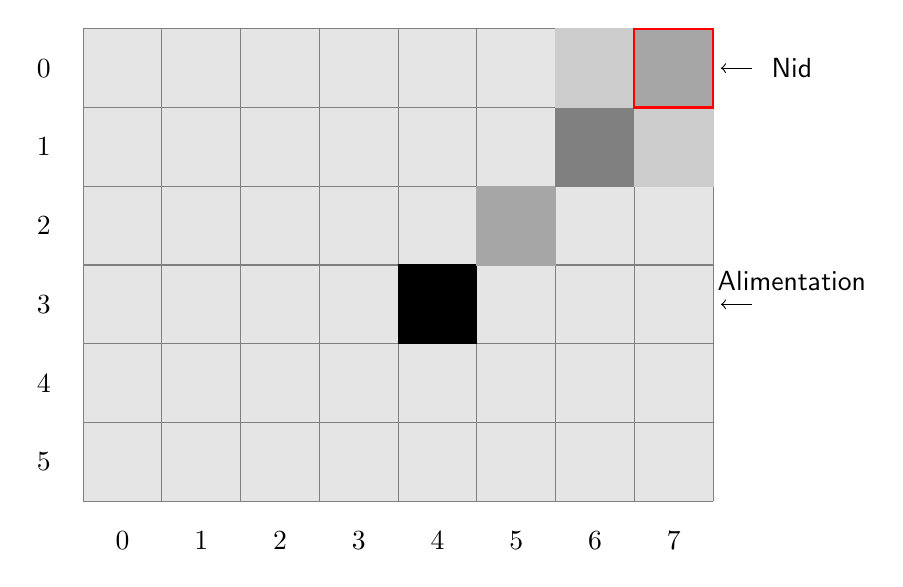
\begin{tikzpicture}
\node at (9,2.8) {\textsf{Alimentation}};
\draw[->] (8.5,2.5) to +(-.4,0);
\node at (9,5.5) {\textsf{Nid}};
\draw[->] (8.5,5.5) to +(-.4,0);
\foreach \x in {0, 1, 2, 3, 4, 5, 6, 7}
  \foreach \y in {0, 1, 2, 3, 4, 5}
  \draw[fill,gray!20] (\x,\y) rectangle +(1,1);
\draw[step=1cm,gray,thin] (0,0) grid (8,6);
\draw[fill] (4,2) rectangle +(1,1);
\draw[fill,gray!70] (5,3) rectangle +(1,1);
\draw[fill,gray] (6,4) rectangle +(1,1);
\draw[fill,gray!70] (7,5) rectangle +(1,1);
\draw[fill,gray!40] (6,5) rectangle +(1,1);
\draw[fill,gray!40] (7,4) rectangle +(1,1);
\foreach \n/\x in {0/.5, 1/1.5, 2/2.5, 3/3.5, 4/4.5, 5/5.5, 6/6.5, 7/7.5}
  \node at (\x, -.5) {\p{\n}};
\foreach \n/\y in {5/.5, 4/1.5, 3/2.5, 2/3.5, 1/4.5, 0/5.5}
  \node at (-.5, \y) {\p{\n}};
\draw[red,thick] (7,5) rectangle +(1,1);
\end{tikzpicture}
\end{center}
\caption{Probabilités de localisation d'un robot avec un marqueur}\label{fig.ant-grid-gray}
\end{figure}

Une fois que la fourmi a atteint le nid, elle se déplace à nouveau au hasard, c'est-à-dire qu'elle choisit un voisin au hasard. En général, une cellule a huit voisins (au-dessus et au-dessous, à gauche et à droite, quatre sur les diagonales), de sorte que la probabilité est $p/8$ qu'elle se trouve dans l'un de ces voisins. Le nid, cependant, se trouve dans le coin et n'a que trois voisins, la probabilité est donc de $p/3$ qu'il se déplace vers l'un d'entre eux. La figure \ref{fig.ant-grid-prob} montre la probabilité de l'emplacement de la fourmi après avoir trouvé la source de nourriture, être retournée au nid et avoir effectué un déplacement aléatoire supplémentaire. Lorsqu'elles sont mises en œuvre par un robot muni d'un marqueur, les cellules présentant une probabilité plus élevée deviennent plus foncées (figure~\ref{fig.ant-grid-gray}).

Que pouvons-nous conclure de ce modèle ?
\begin{itemize}
\item Bien que les fourmis se déplacent au hasard, leur comportement de retour au nid après avoir trouvé la source de nourriture fait que la probabilité de se trouver sur la diagonale est plus élevée que partout ailleurs dans l'environnement. 
\item Puisque les fourmis déposent des phéromones (marques noires) dans chaque cellule qu'elles visitent, il s'ensuit que les marques sur le chemin diagonal entre la source de nourriture et le nid seront plus foncées que les marques sur les autres cellules. Finalement, les marques sur ce chemin seront suffisamment sombres pour que le robot puisse le suivre jusqu'à la source de nourriture sans effectuer d'exploration aléatoire.
\item Puisque le robot visite souvent le nid, les cellules dans le voisinage immédiat du nid auront une probabilité quelque part entre la probabilité uniforme et la probabilité élevée du sentier. Il est donc important de mettre l'accent sur la piste en utilisant des méthodes telles que celles explorées dans l'activité~\ref{act.high-density}.
\end{itemize}

\section[Une machine pour la recherche de chemin]{Une machine à états finis pour l'algorithme de recherche de chemin}\label{s.fsm-ants}
\index{recherche de chemin!fourmis}

Une FSM pour la recherche de chemin par les fourmis est représentée sur la Fig.~\ref{fig.fsm-ant}. Pour gagner de la place, les étiquettes des transitions utilisent des abréviations qui sont expliquées dans le tableau~\ref{tab.abbrev}. Voici une description détaillée du comportement spécifié par ce FSM dans chaque état :

\smallskip

\begin{figure}
\begin{center}
\begin{tikzpicture}[node distance = 3.5cm and 3.8cm,align=left,minimum size=14mm,every loop/.style={min distance=16mm}]
% Nodes
\node[draw,circle] (search) {\p{recherche}};
\node[draw,circle] (follow) [right=of search] {\p{suivre}};
\node[draw,circle] (food) [below=of follow] {\p{alimentation}};
\node[draw,circle] (nest) [below=of search] {\p{aller}\\\p{au nid}};
% Initial state arrow
\draw[->] (-15mm,10mm) to node [above left,xshift=6pt] {\p{vrai} $\leadsto$ \p{avant}} (search);
% Transitions from search
\path[->] (search) edge [loop left] node [below,yshift=-1mm] {\p{mur} $\leadsto$\\\p{turn $90$--$270$,}\\\p{avant}} ();
\path[->] (search) edge [loop above] node {\p{délai d'attente} $\leadsto$\\\p{tourner $0$--$360$,}\\\p{avant}} ();
\path[->,bend left=40] (search) edge node[above,xshift=-2mm,yshift=-3mm] {\p{gris} $\leadsto$  \p{avant}} (follow);
% Transitions from follow
\path[->] (follow) edge [loop above] node[yshift=-1mm] {\p{gris D/G} $\leadsto$\\\p{avant D/G}} ();
\path[->] (follow) edge [loop right] node [below,yshift=-1mm,xshift=-3mm] {\p{gris D\&G} $\leadsto$\\\p{avant}} ();
\path[->] (follow) edge node[above,yshift=-3mm] {\p{délai d'attente} $\leadsto$ \p{avant}} (search);
\path[->,bend left=15] (follow) edge node[left,yshift=4mm,xshift=17mm] {\p{noir} $\leadsto$ \p{--}} (food);
\path[->,bend left=40] (follow) edge node[below,xshift=4mm] {\p{mur} $\leadsto$\\\p{tourner} $450$--$360$, \p{fwd}} (search);
% Transitions from at food
\path[->] (food) edge [loop right] node [below,yshift=-10mm,xshift=-8mm] {\p{direction du nid}\\\p{introuvable} $\leadsto$\\\p{tourner}} ();
\path[->] (food) edge node[below,yshift=2mm] {\p{direction du nid trouvée} $\leadsto$\\\p{se tourner vers le nid}} (nest);
% Transitions from nest
\path[->,bend left=15] (nest) edge node[right,xshift=-23mm,yshift=1mm] {\p{au nid} $\leadsto$ \p{avant}} (search);
\path[->] (nest) edge [loop left] node [above,yshift=1mm] {\p{nid D/G} $\leadsto$\\\p{avant D/G}} ();
\path[->] (nest) edge [loop below] node[left,xshift=-8mm,yshift=4mm] {\p{front du nid} $\leadsto$\\\p{avant}} ();
\end{tikzpicture}
\end{center}
\caption{Machine à états pour tracer un chemin entre une source de nourriture et un nid. Voir le tableau~\ref{tab.abbrev} pour l'explication des abréviations.}\label{fig.fsm-ant}
\end{figure}

\begin{table}[bt]
\caption{Abréviations dans la machine à états}
\label{tab.abbrev}
\begin{tabular}{p{2.5cm}p{7.5cm}}
\hline
Abréviation & Explication \\
\hline
\p{avant} & \p{régler le moteur en avant}\\
\p{avant D/G} & \p{régler le moteur vers l'avant et vers la droite/gauche}\\
& \p{\bfseries fwd et fwd R/L régler également la minuterie sur une période aléatoire}\\
\p{mur} & \p{mur détecté}\\
\p{délai d'attente} & \p{période de la minuterie expirée}\\
\p{gris D/G/D\&G} & \p{gris détecté par les capteurs droit/gauche/les deux capteurs}\\
\p{front du nid/D/G} & \p{nid détecté à l'avant/à droite/à gauche}\\
\p{noir} & \p{noir détecté}\\
\p{direction du nid} & \p{direction de la nourriture vers le nid trouvée ou non trouvée}\\
\p{tourner $\theta_1$--$\,\theta_2$} & \p{tournent aléatoirement dans l'intervalle $\theta_1$--$\,\theta_2$}\\
\p{tourner}&\p{le robot (ou son capteur) tourne}\\
\hline
\end{tabular}
\end{table}

\noindent\textbf{\p{search}:} Dans cet état, le robot recherche au hasard les zones sombres. Il s'agit de l'état initial et la transition \p{vrai $\leadsto$ fwd} spécifie qu'initialement (et inconditionnellement) le robot se déplace vers l'avant et qu'une minuterie est réglée sur une période aléatoire. Lorsque le délai expire (\p{timeout}), le robot effectue un virage aléatoire, se déplace vers l'avant et réinitialise le délai. Ce mouvement aléatoire se poursuit jusqu'à ce que le robot rencontre le mur de la zone ou une marque grise à la surface de la zone. S'il rencontre un mur, il effectue un virage aléatoire en s'éloignant du mur ; nous supposons que le capteur est orienté directement vers l'avant, de sorte que le virage aléatoire doit se faire dans une certaine direction, sur le côté ou à l'arrière du robot. Une fois que le robot a détecté un marquage gris, il passe à l'état \p{suivre}.

\smallskip

\noindent\textbf{\p{follow}:} Les deux auto-transitions situées au-dessus et à droite de cet état sont des transitions qui mettent en œuvre le suivi de ligne (\ref{s.line}). Il existe trois autres transitions : Si un \p{timeout} se produit sans détecter de gris, le robot ne suit plus de ligne et doit retourner à l'état \p{search}. Si le robot rencontre un mur, nous voulons qu'il se détourne, mais nous lui demandons d'abord d'effectuer un tour complet de $360^\circ$ pour vérifier s'il y a un marquage gris à proximité. Par conséquent, la transition inclut l'action \p{turn} $450$--$360$. Comme le nid est situé à côté d'un mur, cette condition est également vraie lorsque le robot retourne au nid. Si le robot détecte un marquage à haute densité (\p{noir}), il conclut qu'il a atteint la source de nourriture et effectue la transition vers l'état \p{à la nourriture}.

\smallskip

\noindent\textbf{\p{at food}:} Enfin, le robot a découvert la source de nourriture. Il doit maintenant retourner au nid. Nous avons spécifié que le nid peut être détecté (Activity~\ref{act.locate-nest}), mais le capteur du robot ne fait pas nécessairement face à la direction du nid. Par conséquent, le robot (ou son capteur) doit tourner jusqu'à ce qu'il trouve la direction du nid. Il se tourne alors vers le nid et passe à l'état \p{goto nid}.

\smallskip

\noindent\textbf{\p{goto nest}:} Cet état est similaire à l'état \p{suivre} en ce sens que le robot avance vers le nid, en tournant à droite ou à gauche si nécessaire pour se déplacer dans la direction du nid. Lorsqu'il atteint le nid, il retourne à l'état \p{recherche}.

\smallskip

Regardez à nouveau la Fig.\ref{fig.ant-result} qui montre une expérience réelle avec un robot exécutant cet algorithme. Nous voyons qu'il y a une forte densité de lignes entre le nid et la source de nourriture, mais qu'il y a aussi une densité relativement élevée de lignes à proximité du nid, pas nécessairement dans la direction de la source de nourriture. Cela peut amener le robot à revenir à une recherche aléatoire au lieu de se diriger directement vers la source de nourriture.

\section{Résumé}

Les algorithmes d'évitement d'obstacles utilisent des algorithmes connus depuis l'Antiquité dans le contexte de la navigation dans un labyrinthe. Lorsqu'ils sont utilisés pour l'évitement d'obstacles, diverses anomalies peuvent faire échouer les algorithmes, en particulier, l'obstacle en forme de $G$ peut piéger un algorithme de suivi de mur. L'algorithme Pledge permet de surmonter cette difficulté.

Une colonie de fourmis peut déterminer un chemin entre son nid et une source de nourriture sans connaître sa position et sans carte en renforçant un comportement aléatoire qui a un résultat positif.

\section{Lecture complémentaire}

Il existe une abondante littérature sur les labyrinthes, que l'on peut consulter en suivant les références de l'article de Wikipédia consacré à \emph{Maze}. L'algorithme de Pledge a été découvert par John Pledge, âgé de 12 ans ; notre présentation est basée sur \cite[Chap.~4]{turtle}. Un projet basé sur les fourmis qui suivent les phéromones est décrit dans~\cite{Mayet2010}.
